\documentclass[10pt]{beamer}
\usepackage{anyfontsize}
\usepackage{minted}
\usepackage[T1]{fontenc}
% \usepackage{inconsolata}

\usepackage[style=british]{csquotes}

\def\signed #1{{\leavevmode\unskip\nobreak\hfil\penalty50\hskip1em
  \hbox{}\nobreak\hfill #1%
  \parfillskip=0pt \finalhyphendemerits=0 \endgraf}}

\newsavebox\mybox
\newenvironment{aquote}[1]
  {\savebox\mybox{#1}\begin{quote}\openautoquote\hspace*{-.7ex}}
  {\unskip\closeautoquote\vspace*{1mm}\signed{\usebox\mybox}\end{quote}}

\title[G-NODE FOSDEM]{G-Node Goes to FOSDEM}
\author{Achilleas Koutsou \& Michael Sonntag}
\date{March 05, 2018}

\graphicspath{{./figures/}{./photos/}}

\begin{document}

\maketitle

\begin{frame}{FOSDEM}
    \begin{center}
        \textbf{F}ree and \textbf{O}pen \textbf{S}ource Software \textbf{D}evelopers' \textbf{E}uropean \textbf{M}eeting
    \begin{figure}
        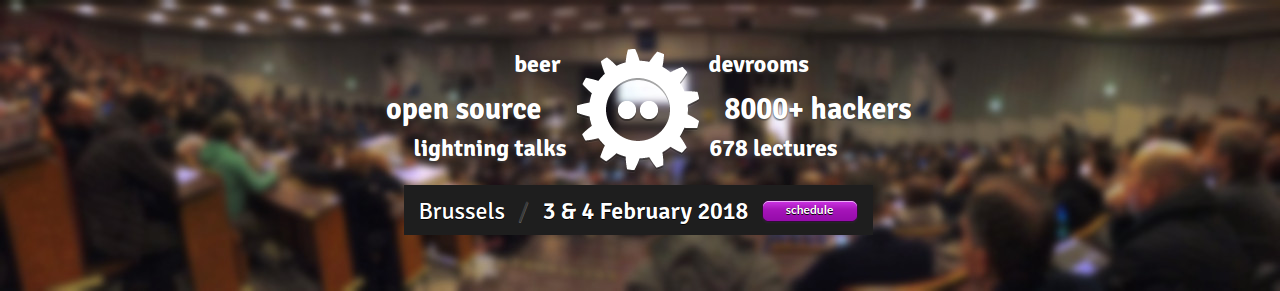
\includegraphics[width=\textwidth]{FOSDEM-banner.png}
    \end{figure}
    \end{center}

\end{frame}

\begin{frame}{FOSDEM}{About}
    Since 2001
    \begin{aquote}{FOSDEM about page}
        [\ldots] a two-day event organised by volunteers to promote the widespread use of free and open source software.
    \end{aquote}

    \begin{itemize}
        \item When: First weekend of February (every year)
        \item Where: ULB Campus du Solbosch Av. F. D. Roosevelt 50 1050 Bruxelles Belgium (every year)
        \item Registration: Free, no registration necessary (every year)
        \item Size: 8000+ estimated (and growing (every year))
    \end{itemize}
\end{frame}


\begin{frame}{NIX}{Resources}
    Resources

    \begin{itemize}
        \item FOSDEM 2018: \url{https://fosdem.org/2018}
    \end{itemize}
\end{frame}

\end{document}
